\documentclass[]{article}
\usepackage{lmodern}
\usepackage[compact]{titlesec}
\usepackage{amssymb,amsmath}
\usepackage{ifxetex,ifluatex}
\usepackage{fixltx2e} % provides \textsubscript
\ifnum 0\ifxetex 1\fi\ifluatex 1\fi=0 % if pdftex
  \usepackage[T1]{fontenc}
  \usepackage[utf8]{inputenc}
\else % if luatex or xelatex
  \ifxetex
    \usepackage{mathspec}
  \else
    \usepackage{fontspec}
  \fi
  \defaultfontfeatures{Ligatures=TeX,Scale=MatchLowercase}
\fi
% use upquote if available, for straight quotes in verbatim environments
\IfFileExists{upquote.sty}{\usepackage{upquote}}{}
% use microtype if available
\IfFileExists{microtype.sty}{%
\usepackage{microtype}
\UseMicrotypeSet[protrusion]{basicmath} % disable protrusion for tt fonts
}{}
\usepackage[margin=1in]{geometry}
\usepackage{hyperref}
\hypersetup{unicode=true,
            pdftitle={Design},
            pdfauthor={Darryl Buswell},
            pdfborder={0 0 0},
            breaklinks=true}
\urlstyle{same}  % don't use monospace font for urls
\usepackage{graphicx,grffile}
\makeatletter
\def\maxwidth{\ifdim\Gin@nat@width>\linewidth\linewidth\else\Gin@nat@width\fi}
\def\maxheight{\ifdim\Gin@nat@height>\textheight\textheight\else\Gin@nat@height\fi}
\makeatother
% Scale images if necessary, so that they will not overflow the page
% margins by default, and it is still possible to overwrite the defaults
% using explicit options in \includegraphics[width, height, ...]{}
\setkeys{Gin}{width=\maxwidth,height=\maxheight,keepaspectratio}
\IfFileExists{parskip.sty}{%
\usepackage{parskip}
}{% else
\setlength{\parindent}{0pt}
\setlength{\parskip}{6pt plus 2pt minus 1pt}
}
\setlength{\emergencystretch}{3em}  % prevent overfull lines
\providecommand{\tightlist}{%
  \setlength{\itemsep}{0pt}\setlength{\parskip}{0pt}}
\setcounter{secnumdepth}{0}
% Redefines (sub)paragraphs to behave more like sections
\ifx\paragraph\undefined\else
\let\oldparagraph\paragraph
\renewcommand{\paragraph}[1]{\oldparagraph{#1}\mbox{}}
\fi
\ifx\subparagraph\undefined\else
\let\oldsubparagraph\subparagraph
\renewcommand{\subparagraph}[1]{\oldsubparagraph{#1}\mbox{}}
\fi

%%% Use protect on footnotes to avoid problems with footnotes in titles
\let\rmarkdownfootnote\footnote%
\def\footnote{\protect\rmarkdownfootnote}

%%% Change title format to be more compact
\usepackage{titling}

% Create subtitle command for use in maketitle
\newcommand{\subtitle}[1]{
  \posttitle{
    \begin{center}\large#1\end{center}
    }
}

\setlength{\droptitle}{-2em}
  \title{Design}
  \pretitle{\vspace{\droptitle}\centering\huge}
  \posttitle{\par}
\subtitle{MSPA PREDICT 455-DL-SEC55}
  \author{Darryl Buswell}
  \preauthor{\centering\large\emph}
  \postauthor{\par}
  \date{}
  \predate{}\postdate{}

\begin{document}
\maketitle

\newpage

\section{1 Introduction}\label{introduction}

This assignment looks to improve on an existing visualization found on
the web by employing best visualization practices.

\section{2 Data}\label{data}

Data for this assessment is based on the Iris flower dataset (Machine
Learning and Systems 2011). This dataset contains measurements of three
classes of flowers. Measurements include the width and height of each
flowers sepal and petal. The three classes of flower include Setosa,
Versicolour, and Virginica.

\section{3 Visualization}\label{visualization}

The visualization which I have chosen to improve on can be found within
an article posted on the R-bloggers website (Turner 2011). The article
demonstrates three R generated plots which focus on showing bivariate
relationships between each variable within the Iris dataset. This
assessment has a particular focus on improving the `Iris Scatterplot
Matrix' visualization presented within this article. The visualization
is shown in Appendix A.

In my opinion, the original visualization has a number of shortcomings:

\begin{itemize}
\tightlist
\item
  The correlation coefficients presented in the matrix are sized by
  coefficient strength and as such, the weakest correlation coefficient
  is too small to be easily read.
\item
  The correlation coefficients presented in the matrix lack polarity.
  That is, the viewer is required to look at the trend line drawn in
  each scatter plot in order to determine whether a relationship is
  positive or negative.
\item
  The dataset does not recognize that there are three class of data
  within the original dataset.
\item
  The included x and y-axis ranges for each scatter plot alternate from
  being located on the left/right, top/bottom of the visualization,
  making any assessment of scale difficult.
\end{itemize}

To improve this visualization, I have constructed a 2x2 grid
visualization. The visualization can also be found in Appendix A. The
top left grid box in this visualization contains some basic data summary
statistics for the dataset, the top right grid box contains a summary of
correlations between each variable, and finally, the bottom two grids
show bivariate scatter plots between petal and sepal sizes.

For the correlation summary visualization, I leveraged a modified
version of the plotcorr function from the `ellipse' package. This
visualization has the benefit of being able to show a simplified
representation of variable correlations using ellipse planes. The actual
correlation coefficients are also shown in this visualization and are
indicated as being positive or negative according to the relationship.
The two scatter plots were generated using the `ggplot2' package. By
coloring each scatter plot according to the class (species), the viewer
is able to get a quick glimpse of the relationship between the
continuous and categorical data types. I managed to find a solution to
allow the two scatter plots to share the same legend.

Ultimately, I found R to be quite limiting in terms of its ability to
translate free floating ideas into a final visualization. Some of the
ideas I had throughout this process were either difficult to implement
(combining embedded with object based graphics into the same grid
visualization), or were not able to be achieved at all (adding an
overlay of comments/speech bubble to the plots to highlight noteworthy
trends or relationships). Clearly the visualizer should weigh the
benefits of using a statistical package such as R to generate their
visualization versus solutions which may provide greater flexibility
such as Powerpoint or direct to canvas graphical programs.

\section{4 Conclusion}\label{conclusion}

The practice of preparing visualizations could be considered more of an
art than of a science. Although there are a number of guides which
dictate `best practice' rules, a great deal of subjectivity still
remains for the visualizer to determine how the visualization should be
structured and delivered. For this assessment, I set out to correct a
number of shortcomings present in a correlation visualization of the
Iris dataset. I believe I was successful in addressing these
shortcomings, however I did find R to be quite limiting in terms of its
flexibility in producing `non-standard' visualizations.

\newpage

\section{Appendix A Figure Output}\label{appendix-a-figure-output}

\subsubsection{Figure A1 Original Iris Scatterplot
Matrix}\label{figure-a1-original-iris-scatterplot-matrix}

\section{\texorpdfstring{\protect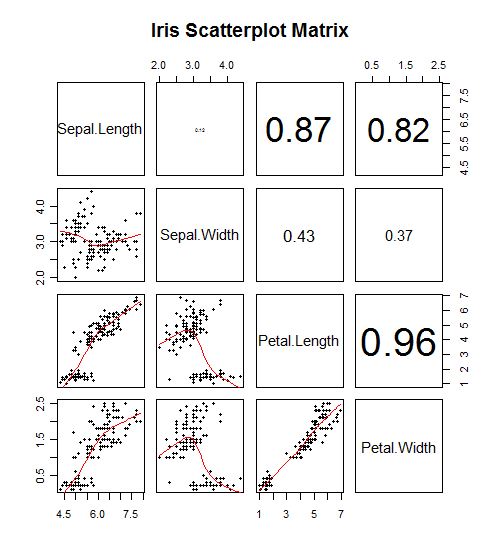
\includegraphics[height=12.50000in]{images/iris_original.png}}{Original Iris Scatterplot Matrix}}\label{original-iris-scatterplot-matrix}

\newpage

\subsubsection{Figure A2 Improved Iris Scatterplot
Matrix}\label{figure-a2-improved-iris-scatterplot-matrix}

\section{\texorpdfstring{\protect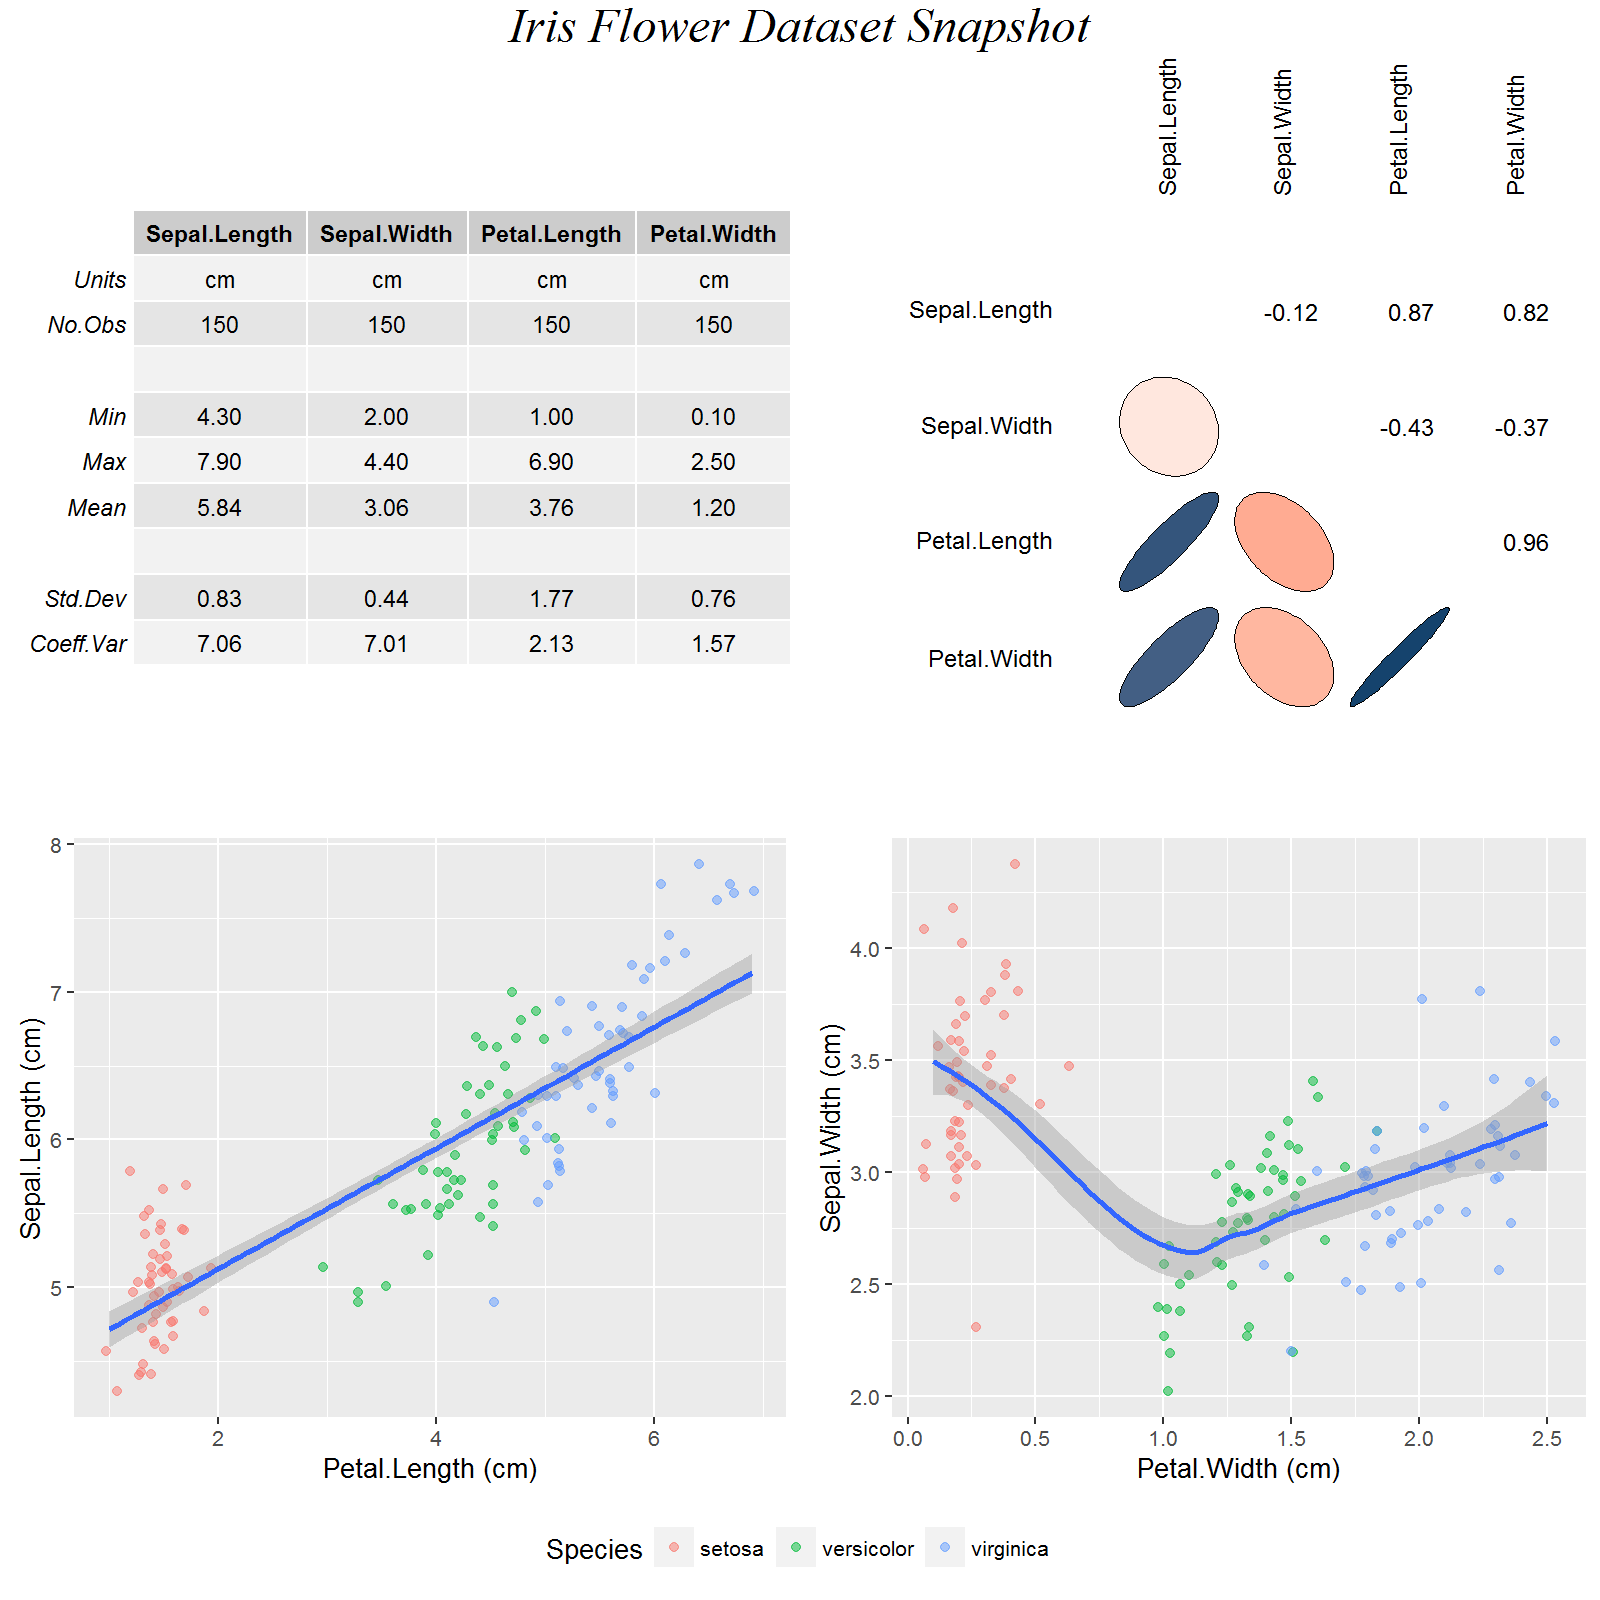
\includegraphics[height=12.50000in]{images/iris_improved.png}}{Improved Iris Scatterplot Matrix}}\label{improved-iris-scatterplot-matrix}

\newpage

\section*{References}\label{references}
\addcontentsline{toc}{section}{References}

\hypertarget{refs}{}
\hypertarget{ref-CEN2011}{}
Machine Learning, Center for, and Intelligent Systems. 2011. ``Iris Data
Set.'' \url{https://archive.ics.uci.edu/ml/datasets/Iris}.

\hypertarget{ref-TUR2011}{}
Turner, S. 2011. ``Scatterplot Matrices in R.''
\url{http://www.r-bloggers.com/scatterplot-matrices-in-r/}.


\end{document}
